\chapter{Implementation}\label{ch:implementation}
With the language design settled in chapter \ref{ch:language_design}, this chapter documents the implementation of the \lang compiler. It touches on how the compiler is structured, justification of the choices made in the process, and documentation with code snippets of the compiler implementation.

\section{Compiler Phases}
The main phases of a compiler are 'Syntax Analysis', 'Contextual Analysis', and 'Code Generation'. In some of these phases, the visitor pattern is mentioned, which is further described in section \ref{lab:visitorPattern}. In this section, these phases are explained and described below.

\subsection{Syntax Analysis}
\noindent\textbf{Lexer:} The first part of the syntax analysis is the lexer, also known as the scanner. The lexer processes the input which is a stream of characters in the source language, and divides them into tokens. If a combination of characters does not match any token in the Lexer, an error is reported \cite{SPO_Topic_3}.\\

\noindent\textbf{Parser:} During Syntax Analysis the tokens get processed into a Parse Tree, using the CFG designed in section \ref{CFGForLang}. The tokens are checked to see if they match the defined grammar rules. If no grammar rules match a sequence of tokens, an error is reported \cite{SPO_Topic_3}. \\

\noindent
\textbf{AST:} Using the Parse Tree, an AST is generated to reduce the size of the tree by simplifying details. The AST nodes are designed in section \ref{AST}. The compiler goes through each grammar rule in the Parse-Tree using the visitor pattern and converts the Parse-Tree into AST nodes \cite{SPO_Topic_3}. 

\subsection{Contextual Analysis}
\noindent \textbf{Symbol Table:} To create a Symbol Table, the AST is iterated through a visitor pattern. 
In the Symbol Table, each scope containing its declared variables is stored. The Symbol Table also checks for scope issues and improper usage of declared variables and reports any error if so \cite{SPO_Topic_3}.\\

\noindent\textbf{Type Checker:} The Type Checker uses the AST and the Symbol Table to check for any type-related errors. This can be done using the visitor pattern \cite{SPO_Topic_3}. \\
%For example, the Type Checker will check if the condition of an if-statement evaluates to a boolean-value. \\

\noindent\textbf{Decorated AST:} When type-checking each node in the AST, additional information like type information and symbol table entries, can be added, generating a decorated AST. However, it is not necessary to create a decorated tree. It depends on the requirement for the compiler \cite{SPO_Topic_3}.

\subsection{Code Generation:} Finally the compiler goes through Code Generation. Code Generation once again uses the visitor pattern. In this phase, instructions based on the decorated AST nodes are generated. These instructions get translated to the target language of the compiler \cite{SPO_Topic_3}.

\section{\lang compiler} \label{peakCompiler}
To create the \lang compiler, these three compiler phases are implemented. The rest of this chapter will describe the implementation of syntax analysis, contextual analysis, and code generation. \\

\begin{figure}[H] 
    \begin{center}
        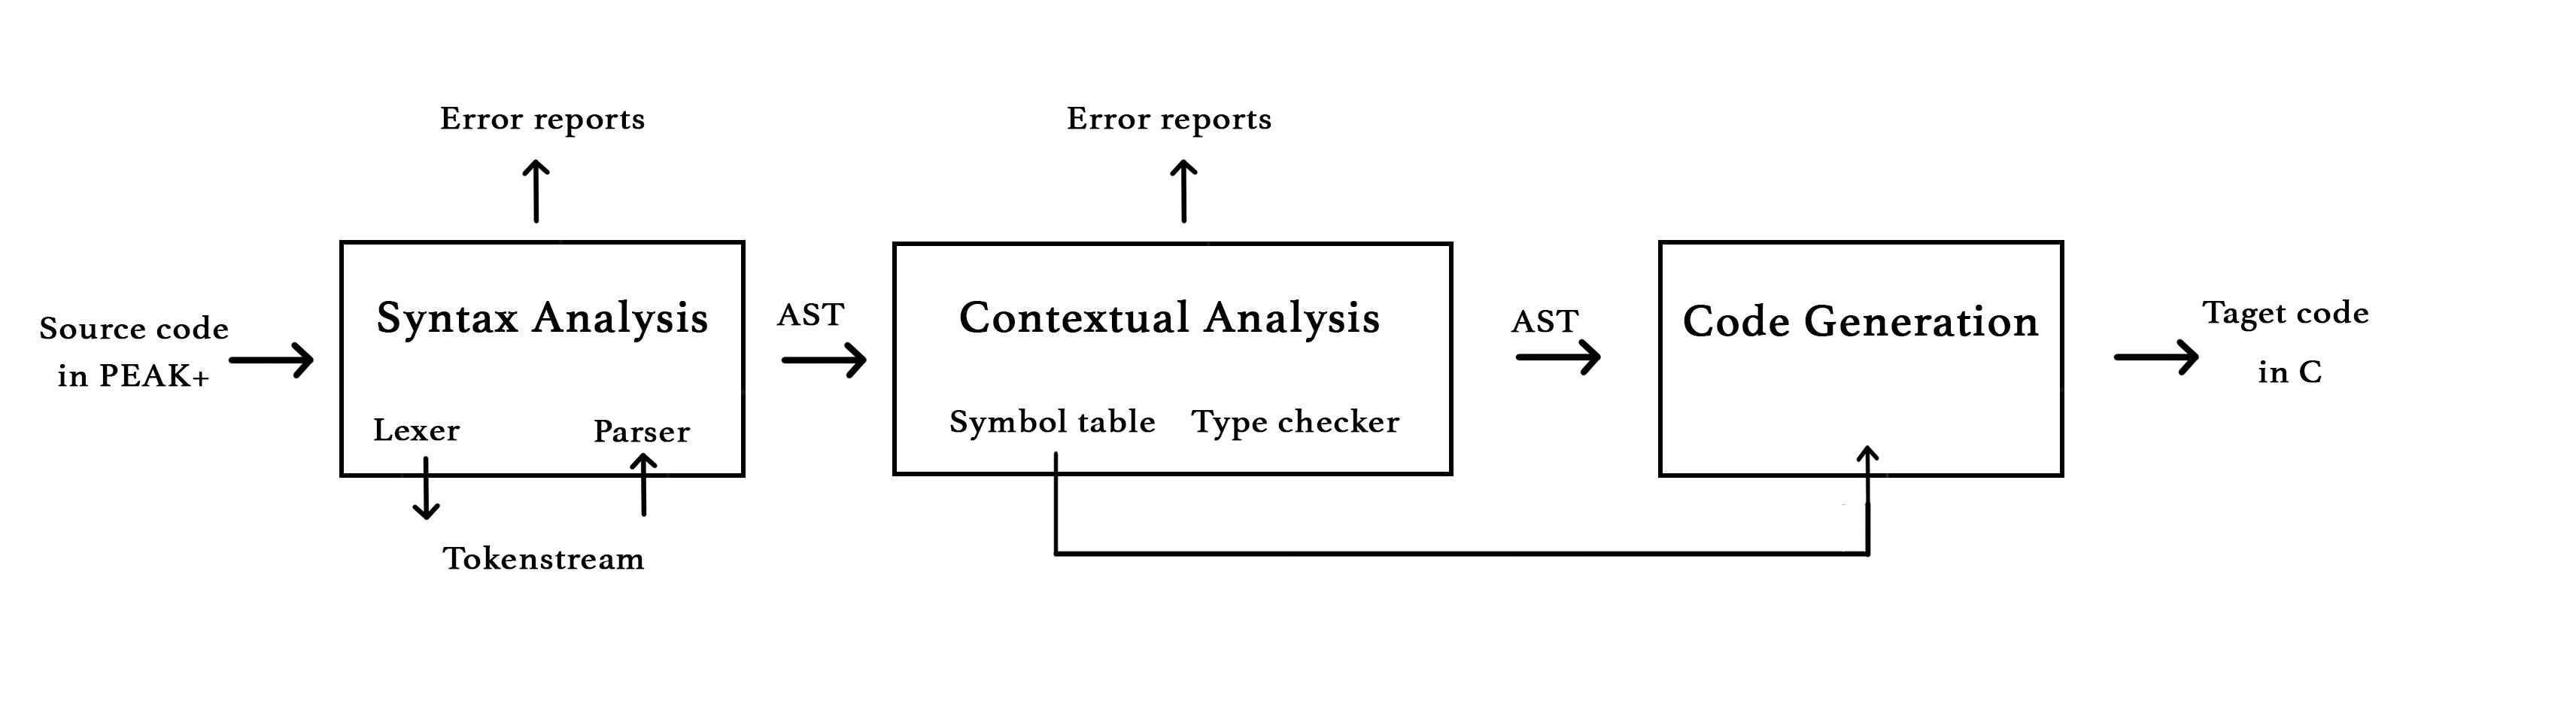
\includegraphics[width=1\textwidth]{Files/Billeder: Impl/OverviewCompiler.jpg}
    \end{center}
    \caption{Overview of the PEAK+ compiler}
    \label{I:Figurue:PEAKCompiler}
\end{figure}

\noindent As displayed in figure \ref{I:Figurue:PEAKCompiler} which shows an overview of the \lang compiler, the input to the lexer is the source code written in \lang. The lexer generates the token stream that the parser uses to generate the AST. Then the scope rules are checked in the symbol table, followed by type checking. The \lang compiler will not generate a decorated AST in the contextual analysis phase. Since \lang is a simple language, there is no need for decorating the AST before translating it into the target code. The target code for \lang is the C programming language. One of the reasons C is chosen is because of its flexibility, which makes it easier to adjust to the semantics of \lang, more details on the reasons behind C as the target code is explained in section \ref{I:CodeGeneration}.

\subsection{Deciding Compiler Language} \label{I:TargetLanguage}
In order to best implement a visitor pattern later on in development, an object-oriented language is needed. The visitor pattern is explained further in section \ref{lab:visitorPattern}. For this reason, the \lang compiler is going to be developed in C\#. This is also because C\# is a language that the group is acquainted with as well as how the project organization works in C\#. 

\section{Syntax Analysis}\label{I:SyntaxAnalysis}
Syntax Analysis is the first phase of the compiler which ends up generating an Abstract Syntax Tree (AST). This section will cover the theory of the parser algorithm followed by the implementation in the \lang compiler including the Parser Generator, and how the AST has been built. 

\subsection{Parsing Theory}
When a compiler translates source code, the parser defines the structure of the code by producing a parse tree. The basis for creating the parse tree is the token stream created by the lexer. The Lexer converts the source code characters into specified tokens. Lexical grammar uses regular expressions to define the grammar rules of a token. As displayed in figure \ref{I:Figure:ParsetreProcess}, the lexer, for example, translates the source code "12 + 23" into the \textit{Num}, \textit{Plus}, and \textit{Num} tokens. The parser uses this token stream to produce the parse tree by using the correlated CFG production rules. Implicit in the displayed example, a lexer rule will exist, specifying that a sequence of digits corresponds to the \textit{Num} token, the plus symbol corresponds to the \textit{Plus} token, and that the correlated CFG production rules say that a program consists of an \textit{expr} and that a \textit{expr} can be a \textit{Num Plus Num} \cite{ParsingGuide}. 

\begin{figure}[H] 
    \begin{center}
        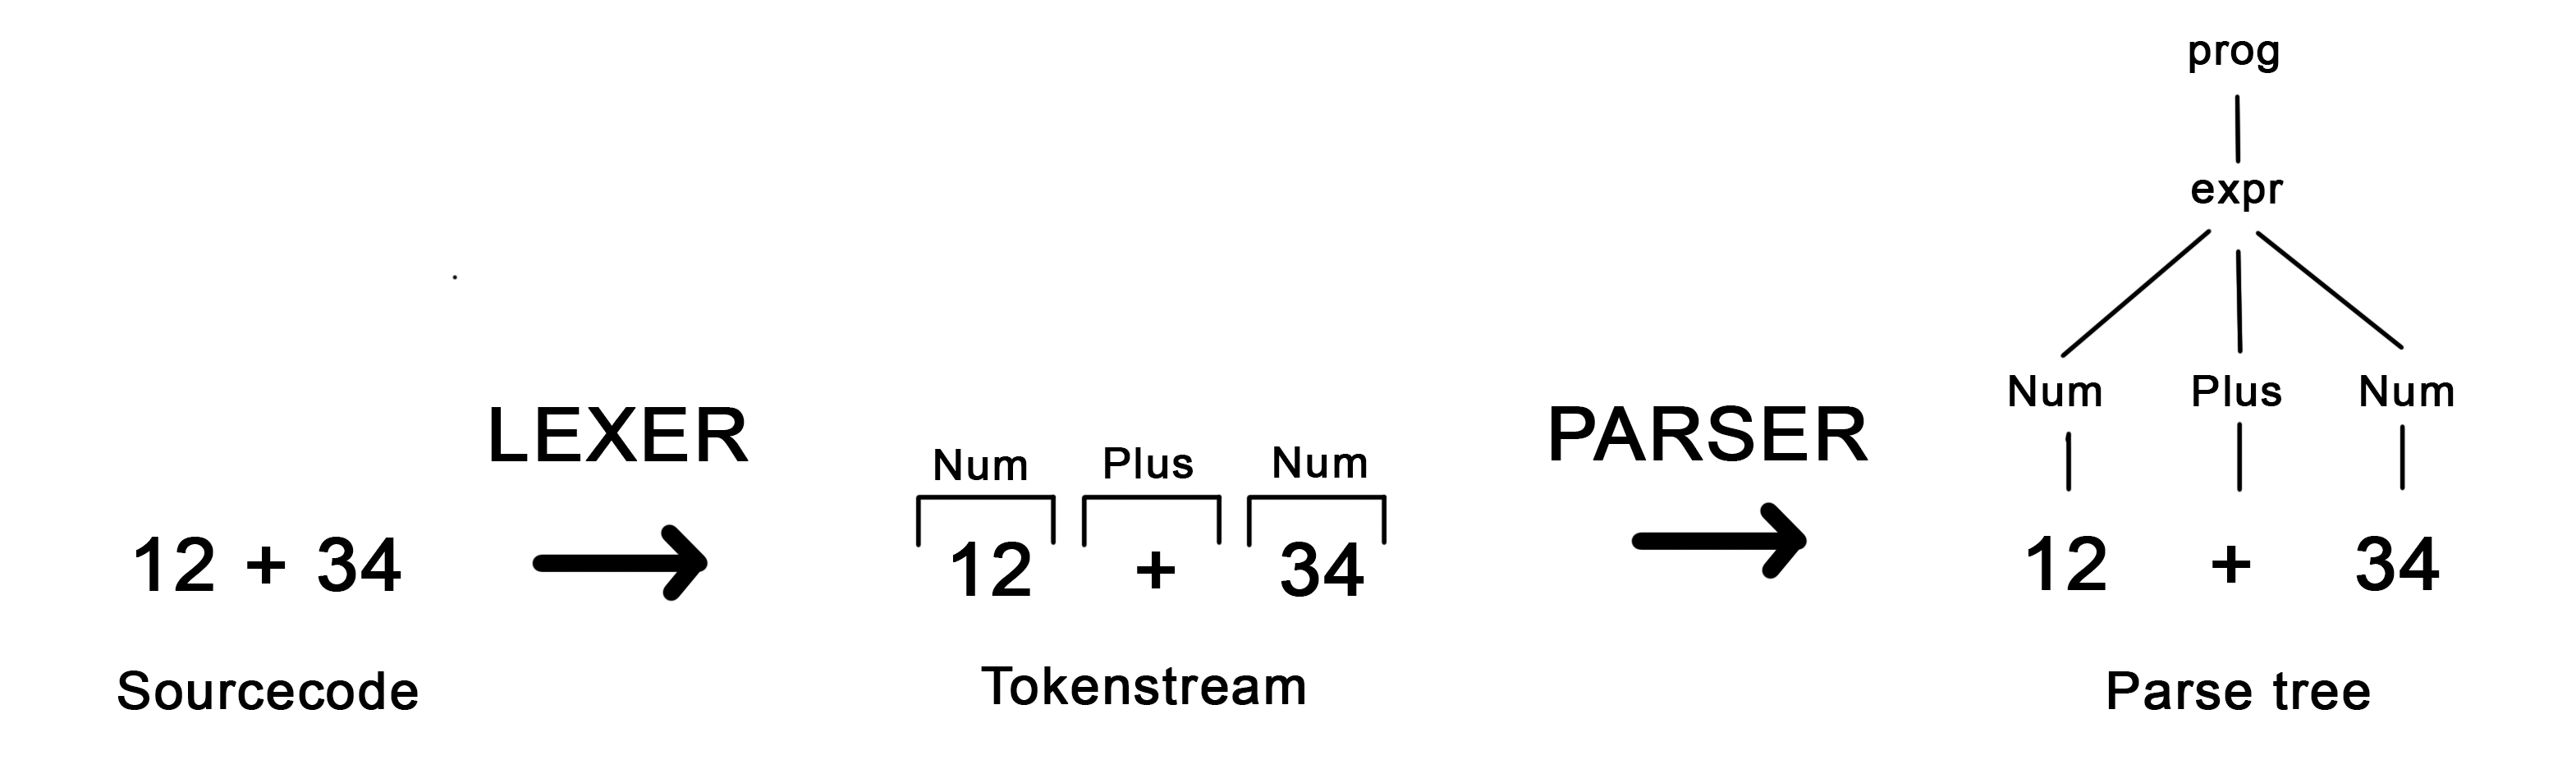
\includegraphics[width=1\textwidth]{Files/Billeder: Impl/parsing kopier.jpg}
    \end{center}
    \caption{An example of the process of translating source code into a parse tree}
    \label{I:Figure:ParsetreProcess}
\end{figure}

\noindent
By generating the parse tree, the parser checks the syntactic correctness of the source code. If the source code consists of syntax errors, error reports will be thrown. An example of syntactically correct but semantically incorrect code is displayed in listing \ref{list:SyntaxCodeFail}. The parser will not produce any errors, since the structure of the code is correct. But if the code is executed, it will fail since the variable x is not declared \cite{ParsingGuide}. 

\begin{lstlisting}[language = csharp, firstnumber=0, label={list:SyntaxCodeFail},caption=example of code with correct syntax but wrong semantics.]
int y = 10;
int sum = x + y;
\end{lstlisting}

\noindent
A parse tree is also called a concrete syntax tree (CST) and is traversed, from the root node of the tree, down to its subtrees representing smaller pieces of the code. The same principle applies to the AST, except that the CST is represented using the concrete syntax while the AST is more simplified and has fewer details that are not relevant for generating code \cite{ParsingGuide}. The difference between the two trees can be seen in figure \ref{I:Figure:ParseAST}. \\

\begin{figure}[H] 
    \begin{center}
        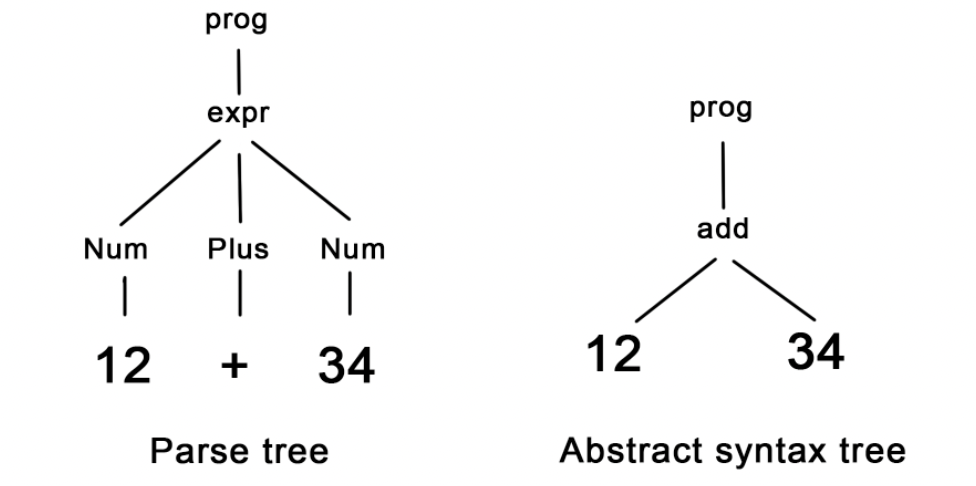
\includegraphics[width=0.7\textwidth]{Files/Billeder: Impl/parsetoAST.png}
    \end{center}
    \caption{Examples showing the difference between a CST and an AST}
    \label{I:Figure:ParseAST}
\end{figure}

\noindent
There are two approaches to parsing: top-down and bottom-up. A top-down parser traverses the tree from the root node until each leaf is visited. These are also known as LL(K) parsers (\textbf{L}eft-to-right read of input, \textbf{L}eftmost derivation). The k indicates the amount of lookahead the algorithm has, meaning how many tokens the parser has to include in its decisions of what grammar rule to follow. LL parsers are easy to implement but less efficient because they cannot handle left recursion grammar rules. However, there will always be an equivalent non-recursive grammar to a left recursive grammar, but the rewritten grammar rules can be more complex to understand, or need more lookaheads than the recursive grammar \cite{ParsingGuide}. \\

A bottom-up parser starts from the lowest part of the tree, ending at the root. The LR (\textbf{L}eft-to-right read of the input, \textbf{R}ightmost derivation) parser is a Bottom-up parser and is harder to implement, but can handle most grammars like left recursion. Both LL and LR parsers use parse tables that store information about the next action to take. For LR parsers, these tables can become large and complex. LALR (Look-Ahead, Left-to-right) is a variant of the LR parser and attempts to address the LR parsers issue by having large table sizes be more compact at the cost of potential conflicts with look-ahead \cite{ParsingGuide}. 

\subsection{Deciding Parser Tool}
Generating the parser can be done by hand or by using a parser generator tool. Using a tool can be faster and more accurate, especially with larger languages. A tool helps to reduce errors in the parser but often has some requirements for the grammar, like having to be LL(1). However, by generating the parser by hand, the developer has more control over how to handle the special requirements. Though, if the language's grammar is large and complex, it is a difficult and time-consuming task to write the parser by hand, leading to errors in the parser. Even though \lang is not that complex, our learning curve in this project means that changes probably would occur along the way. Because of the time consumption of having to rewrite the parser by hand several times, combined with our missing experience in writing a parser, we decided that a tool would be the appropriate choice. There are many different parser generators, and we researched JavaCup, SableCC, and ANTLR. \\

JavaCUP is an LALR bottom-up parser and generates a parser written in Java. Both SableCC and ANTLR are LL(k) and can generate a parser in multiple different languages. We prefer writing code in C\# and therefore the choice is between SableCC and ANTLR. After experimenting with getting both tools to work, ANTLR is the first to successfully work and to show a visual parse tree. In view of getting the parsing process started, ANTLR is therefore chosen as the parser generator. ANTLR can handle left recursion, and is an LL(*) parser meaning it can handle any amount of lookahead tokens \cite{ParsingGuide}.
%The source code for the \lang compiler can be found in the project GitHub repository called "P4-project" \cite{p4-project-rep}.

\subsection{Lexer}
ANTLR provides the ability to perform lexical analysis if it receives a lexer. Because of this, we are able to take our CFG and transform all terminal rules into keywords stored in the lexer. Some of the same terminal rules appear multiple times in the CFG, and therefore it is now easier to change all appearances of a terminal rule at once. Examples of keywords can be seen in listing \ref{list:Lexer_Example} for various list operations. In the lexer, definitions of regular expressions can be made. ANTLR uses different characters in its regular expressions compared to what normally is used. ANTLR for example uses \textit{\~}\ instead of \textit{\^} for excluding characters. Regular expressions are e.g. used in \lang for string values. In \lang, a string value starts with \textit{"} followed by any character which is not a \textit{"} and ends with \textit{"}. In ANTLR this regular expression can be seen in listing \ref{list:Lexer_Example} as 'STR' as well as some examples of other lexer rules. The full lexer can be seen in appendix \ref{list:ANTLR LEXER}.

\begin{lstlisting}[label={list:Lexer_Example}, captionpos=b, caption=Part of \lang's Lexer - CobraCompiler/ExprLexer.txt]
LISTADD: 'Add';
LISTIDXOF: 'IndexOf';
LISTREPLACE: 'Replace';
LISTVALOF: 'ValueOf';

COMM: 'comment:'~(';')*;
STR: '"' (~'"')* '"';
DEC: ('+' | '-')? [0-9]+'.'[0-9]+; 
INT: ('+' | '-')? [0-9]+ ;
ID: [a-zA-Z_][a-zA-Z_0-9]* ; 
WS: [ \t\n\r\f]+ -> skip ; 
\end{lstlisting}

\subsection{The Visitor Pattern}
\label{lab:visitorPattern}
In order to traverse a tree like the CST, a visitor pattern is required. A visitor pattern utilizes a depth-first search method to traverse the tree. It solves the problem of having to modify each class in a larger class structure whenever a change needs to be implemented. Instead, all visitor methods are contained within one class, and therefore only the functions have to be modified. This pattern is used in multiple phases of the \lang compiler, like when building the AST, creating the symbol table, type-checking, and generating the target code. Based on the context, a visit function in the pattern can return something different. For example, when building the AST, each visit function can return an AST node in order to build upon the AST \cite{VisitorWIKI}. An example of how the visitor pattern visits nodes using the depth-first search algorithm can be seen in figure \ref{fig:VisitorPattern_Example}.

\begin{figure}[H] 
    \begin{center}
        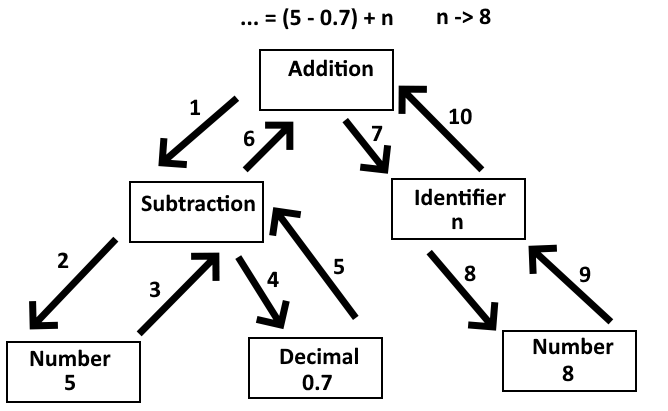
\includegraphics[width=0.6\textwidth]{Files/Billeder: Impl/VisitorpatternExample.png}
    \end{center}
    \caption{Example of the visitor pattern. The numbers above the arrows show which order the nodes are visited}
    \label{fig:VisitorPattern_Example}
\end{figure}

\subsection{Building the Abstract Syntax Tree}
Using ANTLR generates multiple classes including \textit{ExprParser}, \textit{ExprLexer}, and \textit{ExprParserBaseVisitor}. The order in which ANTLR generates the parser can be seen in listing \ref{list:Program_Parser}. First ANTLR uses an \textit{AntlrInputStream} class in order to turn the input into a stream of characters that ANTLR can use, seen on line 28. This stream of characters is used to instantiate a new \textit{ExprLexer} class which is assigned to the lexer variable on line 29. The lexer is then given to a \textit{CommonTokenStream} class which converts the lexer into tokens for the parser. This can be seen on line 30. The returned token stream is given to \textit{ExprParser} which finally generates the parser on line 31. From the parser, the start-node can be retrieved, which in our CFG is '\textit{program}'. This root is assigned to a variable called '\textit{cst}' (concrete syntax tree) on line 35. The '\textit{cst}' is required in order to build the AST.

\begin{lstlisting}[language = csharp, label={list:Program_Parser},firstnumber=28,caption=SymbolTable Class - CobraCompiler/Program.cs]
var inputStream = new AntlrInputStream(new StringReader(exprText));
var lexer = new ExprLexer(inputStream);
var tokenStream = new CommonTokenStream(lexer);
var parser = new ExprParser(tokenStream);
.
.
.
var cst = parser.program();
\end{lstlisting}

\noindent
Before building the AST, classes for each of the possible nodes must be created. '\textit{ASTNodes}' is a class that is created to contain these as well as the datatypes in \lang stored as an enumeration. These nodes are designed in section \ref{ASTDesign}. Each node inherits from an abstract class '\textit{ASTNode}' and through this, all nodes contain a property '\textit{Line}' which represents the line in the code where the node originates from. This property is used to inform the user where an error stems from if one occurs. \\

\noindent An example of the '\textit{AssignNode}' can be seen in listing \ref{list:ASTNodes}. In \lang, an assignment is written as $identifier = expression$. '\textit{AssignNode}' inherits '\textit{CommandNode}' since an assignment is a command. It contains an \textit{IdentifierNode} on line 54 and an \textit{ExpressionNode} on line 55.

\begin{lstlisting}[language = csharp, label={list:ASTNodes}, firstnumber=52, caption=SymbolTable Class - CobraCompiler/ASTNodes.cs]
internal class AssignNode : CommandNode
{
    public IdentifierNode Identifier { get; set; }
    public ExpressionNode Expression { get; set; }
}
\end{lstlisting}

\noindent
ANTLR generates the '\textit{ExprParserBaseVisitor}' class which is used by a class '\textit{BuildASTVisitor}'. It is used for building the AST by having '\textit{BuildASTVisitor}' inherit from it. '\textit{ExprParserBaseVisitor}' provides a visitor pattern for going through the symbols in the parse tree. It is a generic class and the generic type given is the return type of all visitor implementations of the class. This is in our case the class '\textit{ASTNode}'. The class contains unique visit methods for each non-terminal in \lang's CFG, as well as a general '\textit{Visit()}' method. In each of these methods, you are able to access the non-terminal '\textit{context}' which is used to get its children. The context can also be used to retrieve the line in which a rule occurred that can be stored in an AST node. The children can be used on the '\textit{Visit()}' method to visit the non-terminals children.\\

\noindent Using this, we can visit all children in the parse tree and return the correct ASTNodes. Each unique visit method has the following structure: 
\begin{itemize}
    \item All children are initialized at the top using the symbol's context
    \item If a node is to be returned, this also gets initialized here as '\textit{outputNode}'
    \item  One or more if-statements check for necessary syntax rules and visit the children
    \item At the bottom, the \textit{outputNode}'s properties are assigned, and it is returned
\end{itemize}

\noindent In order to test if '\textit{BuildASTVisitor}' returns the correct output, a '\textit{prettyPrint()}' function is run every time a new node is added to the AST. In order to correctly print the nodes at their respective levels of the AST, an indentation function '\textit{incrIndent()}' can be called. This function increments indentation for the next time a node is pretty printed. A function '\textit{decrIndent()}' decreases indentation again. An example of how it looks in the terminal, as a result of the implemented indentation can be seen in figure \ref{fig:pretty_print}. Because of time pressure, the pretty printer is not being maintained in the second iteration as it is mostly used to check if the output of the \textit{BuildASTVisitor} matches the source code. In the second iteration, we use debugging features to ensure that the resulting AST match.

\begin{figure}[H] 
    \begin{center}
        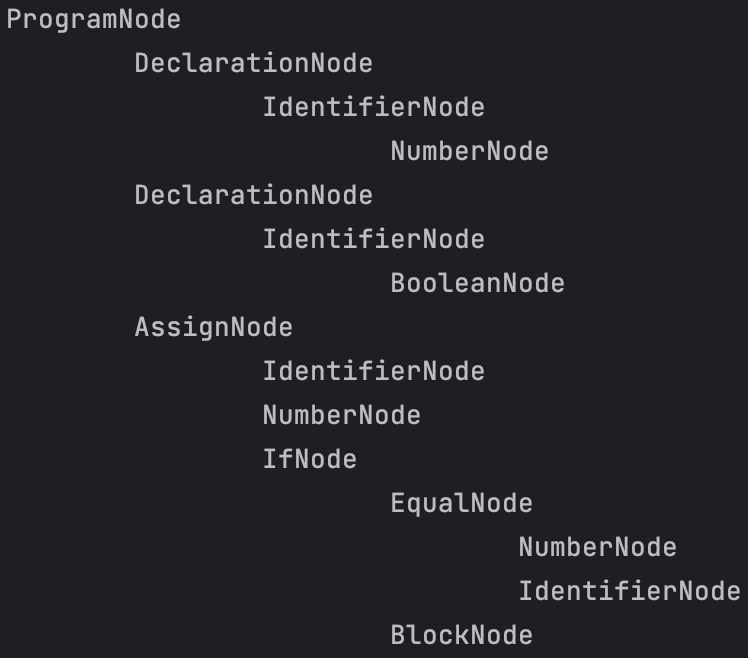
\includegraphics[width=0.5\textwidth]{Files/Billeder: Impl/pretty_print.png}
    \end{center}
    \caption{Pretty print example.}
    \label{fig:pretty_print}
\end{figure}

\noindent
An example of one of the visit functions can be seen in listing \ref{list:BuildASTVisitor}. This example is of a declaration rule in \lang's CFG which has the following structure: $dcl -> type \ ID \ ass \ SEMI;$. In the function, all children are initialized at the top on lines 139-142 as well as the node to return on line 144, which is a declaration node. On lines 149-152 an if-statement checks that the syntax is correct. Since a declaration-node contains an identifier-node we initialize this on line 154. An identifier node has a type node that is visited on line 159 and returned. This type node is assigned to the identifier node on line 160. On line 162, the declaration is checked for any assignments, since it is possible in \lang to have a declaration without any assignments. This assignment is assigned as an 'expression' to the '\textit{outputNode}' on line 167. The identifier node is also assigned on line 145 and the output is returned on line 170.

\begin{lstlisting}[language = csharp, firstnumber=132, label={list:BuildASTVisitor},caption=BuildASTVisitor Class - CobraCompiler/BuildASTVisitor.cs]
public override ASTNode VisitDcl([NotNull] ExprParser.DclContext context)
{
    //outputNode = DelcarationNode
    //visit(type) -> gets TypeNode
    //visit(ass) -> gets ExpressionNode
    //Type and Expression is assigned to an identifierNode
    //The identifierNode is assigned to the OutputNode
    var type = context.type();
    var ID = context.ID();
    var ass = context.ass();
    var SEMI = context.SEMI();

    var outputNode = new DeclarationNode() { Line = ass.start.Line };

    prettyPrint("DeclarationNode", context);
    incrIndent();

    if ((type != null) &&
        (ID != null) &&
        (ass != null) &&
        (SEMI != null))
    {
        var identifier = new IdentifierNode() { Line = ID.Symbol.Line };
        prettyPrint("IdentifierNode", context);
        incrIndent();

        identifier.Name = ID.ToString();
        var typeNode = (TypeNode)Visit(type);
        identifier.TypeNode = typeNode;

        if (ass.ChildCount > 0)
        {
            outputNode.Expression = (ExpressionNode)Visit(ass);
        }

        outputNode.Identifier = identifier;
    }

    decrIndent();
    return outputNode;
}
\end{lstlisting}

\newpage
\section{Contextual Analysis}\label{I:ContextualAnalysis}
Contextual Analysis is the phase of the compiler that usually "decorates" the AST to make a Decorated AST. It uses the Symbol Table and Type Checking to add any additional information which can for example be type information when performing type conversion. After the decorated AST is made the compiler enters the Code Generation phase. In \lang, we did not add type information to the AST until the second iteration, as it is necessary for the code generation to recognize for example if an addition-node is concatenating strings or adding two numbers.

\subsection{Symbol Table}
The symbol table created for \lang is developed in C\#. It is created using a '\textit{Scope}' class which represents the scopes of the program. This class can be seen in listing \ref{list:ScopeClass} and contains a stack of dictionaries, used for storing symbols and a reference to the scope '\textit{Parent}' (meaning its outer scope). It also stores a reference to the Block Node tied to the scope. In order to get a symbol from the dictionary when knowing its ID, the dictionary's key is the symbol's ID. This helps to get the symbol in constant time, which is more efficient for the compiler than iterating through all symbols until it finds a match. The Symbol class in listing \ref{list:SymbolClass} defines the properties of a symbol, which includes its name, type, and reference to the declaration node. The Type property is of type \textit{TypeEnum}, which is an enumerator that defines the possible types of symbols: number, text, boolean, decimal,  list\_number, list\_text, and list\_boolean.\\
The scope rules which the symbol table manages are described in section \ref{sec:scope_rules}.

\begin{lstlisting}[language = csharp, firstnumber=28, label={list:ScopeClass},caption=Scope Class - CobraCompiler/SymbolTable.cs]
public class Scope
{
    public Scope()
    {
        Symbols = new Dictionary<string, Symbol>();
    }
    public Dictionary<string, Symbol> Symbols { get; set; }
    public Scope Parent { get; set; }
    public BlockNode Block { get; set; }
}
\end{lstlisting}

\begin{lstlisting}[language = csharp, firstnumber=21, label={list:SymbolClass},caption=Symbol Class - CobraCompiler/SymbolTable.cs]
public class Symbol
{
    public TypeEnum Type { get; set; }
    public string Name { get; set; }
    public ASTNode Reference { get; set; }
}
\end{lstlisting}

\noindent
The SymbolTable class in listing \ref{list:SymbolTableClass} builds and stores the symbol table. Besides its 'Visit()' functions, the class provides six methods \textit{BuildSymbolTable()}, \textit{ProcessNode()}, \textit{NewScope()}, \textit{ExitScope()}, \textit{Insert()}, and \textit{Lookup()}. The \textit{BuildSymbolTable()} method takes the root of the AST as its input and processes each node in the tree using the visitor pattern. \\

The \textit{NewScope()} method is used when visiting a new block when building the symbol table. It takes a \textit{BlockNode} as a parameter, creates a new scope, and pushes it onto a stack. This stack keeps track of the current scope by storing it at the top. If possible, the parent of the scope is also set. The scope is also stored in a separate dictionary where each scope can be accessed using its \textit{BlockNode}. Finally, the blockNode which belongs to the now current scope, is stored.\\

The \textit{ExitScope()} method pops the top element of the scope stack to represent exiting a scope. This method is called when exiting a scope during the symbol table creation. \\

The Insert method takes a string \textit{name} and a \textit{TypeEnum} as its inputs and adds a new symbol to the current scope at the top of the stack. Insert is called when visiting a declaration node, as the newly declared variable needs to be stored in the symbol table. \\

The Lookup method takes a string \textit{name} and a \textit{BlockNode}. It starts at the scope belonging to the \textit{BlockNode} and searches outwards through each scope's dictionary for the requested symbol and returns it if found. If the symbol is not found, \textit{null} is returned and an error is reported. This function is called when meeting an Identifier node in the AST, which represents already declared variables.

\begin{lstlisting}[language = csharp, firstnumber=39, label={list:SymbolTableClass},caption=SymbolTable Class - CobraCompiler/SymbolTable.cs]
public class SymbolTable : ASTVisitor<ASTNode?>
{
    public Dictionary<BlockNode, Scope> _scopes;
    public Stack<Scope> _stackScopes;
    private ErrorHandler symbolErrorhandler;
    public BlockNode _currentBlock;
    .
    .
    .
    public SymbolTable(ErrorHandler errorHandler)
    {
        symbolErrorhandler = errorHandler;
        _scopes = new Dictionary<BlockNode, Scope>();
        _stackScopes = new Stack<Scope>();
    }
    public SymbolTable BuildSymbolTable(ASTNode astRoot)
    {
        Visit((ProgramNode)astRoot);
        return this;
    }
\end{lstlisting}

\begin{lstlisting}[language = csharp, firstnumber=232, label={list:Visit},caption=Visit(DeclarationNode node) - CobraCompiler/SymbolTable.cs]
public override ASTNode? Visit(DeclarationNode node)
{
    if (_reservedKeywords.Contains(node.Identifier.Name))
        node.Identifier.Name = $"{node.Identifier.Name}_";

    var sym = Lookup(node.Identifier.Name, _currentBlock);

    string underscores = "";
    while (sym != null)
    {
        underscores += "_";
        sym = Lookup($"{node.Identifier.Name}{underscores}", _currentBlock);
    }

    node.Identifier.Name += underscores;
    Insert(node.Identifier.Name, node.Identifier.TypeNode.Type, node);
    Visit(node.Expression);
    return null;
}
\end{lstlisting}

\noindent
\textit{NewScope()} in listing \ref{list:NewScope} creates a new scope in the symbol table. It takes a block node on line 75, which is associated with the scope, and assigns it to a new scope on line 78. If any scopes already exist, the scopes parent is assigned to the current scope at the top of the stack on lines 80-81. The scope is pushed onto a stack of scopes and added to a dictionary of scopes on lines 83-84. The current block is then updated to refer to the new scope block on line 85. The method uses \textit{\_stackScopes.Peek()} on the dictionary on lines 81 and 85 to retrieve the top element which is the current scope. This function is called when entering a new block of code, such as a function or loop. Variables declared within this block will only be visible within this scope and any nested scopes.

\begin{lstlisting}[language = csharp, firstnumber=75, label={list:NewScope},caption=NewScope() - CobraCompiler/SymbolTable.cs]
private void NewScope(BlockNode blockNode)
{
    var scope = new Scope();
    scope.Block = blockNode;

    if (_stackScopes.Count > 0)
        scope.Parent= _stackScopes.Peek();

    _scopes.Add(blockNode, scope);
    _stackScopes.Push(scope);
    _currentBlock = _stackScopes.Peek().Block;
}
\end{lstlisting}

\noindent
The method \textit{ExitScope()} in listing \ref{list:ExitScope} exits the current scope in the symbol table. It pops the top dictionary from the scope stack using the \textit{Pop()} method, effectively removing it from the symbol table on line 90. It also updates the current block to be that of the new current scope after popping the stack on lines 92-93. It does this if the block is not of type program-node as you can not go further out than the program-node. This method is called when exiting a block of code.

\begin{lstlisting}[language = csharp, firstnumber=89, label={list:ExitScope},caption=ExitScope() - CobraCompiler/SymbolTable.cs]
private void ExitScope()
{
    _stackScopes.Pop();
    if (_currentBlock is not ProgramNode)
        _currentBlock = _stackScopes.Peek().Block;
}
\end{lstlisting}

\noindent
The method \textit{Insert()} in listing \ref{list:Insert} inserts a new symbol into the symbol table. It takes three arguments: the name of the symbol, its type represented by a \textit{TypeEnum}, and the node of the declaration on line 98. Because of the scope rules defined in chapter \ref{ch:language_design}, the same name for a variable can not be defined within the same scope, only in separate scopes. Therefore \textit{Insert()} checks if the current scope contains the name of the variable being inserted on line 100. If it already exists, an error will be reported on line 102. If this is not the case, it adds a new entry to the dictionary using the name parameter as the key and a new \textit{Symbol} object as the value with all the arguments given on line 106.

\begin{lstlisting}[language = csharp, firstnumber=98, label={list:Insert},caption=Insert() - CobraCompiler/SymbolTable.cs]
public void Insert(string name, TypeEnum type, ASTNode node)
{
    if (_stackScopes.Peek().Symbols.ContainsKey(name))
    {
        SymbolError(node, $"The variable '{name}' is defined twice within the same scope.");
        return;
    }

    _stackScopes.Peek().Symbols.Add(name, new Symbol 
    { 
        Name = name, Type = type, Reference = node
    });
}
\end{lstlisting}

\noindent
\textit{Lookup()} in listing \ref{list:Lookup} searches for- and returns a symbol in the symbol table. It takes two arguments being the name of the symbol to look up and a block on line 114. The method first gets the scope associated with the block given on line 116. It enters a while loop checking that the scope has a value on line 118. It then uses a for each to loop through the scopes symbols on line 120. It checks if the current symbol's name matches the name given on line 122. If this is the case, it returns the current symbol on line 124. If the symbol is not found in the scope symbols the scope gets updated to be its own parent on line 128. If the symbol is not found, the method returns \textit{null} on line 130.\\

This method is called when needing to find a symbol associated with a variable name in order to for example look up the type of the variable that has been previously declared. The function can also be used to detect errors, such as when attempting to use an undeclared variable, as giving the name of an undeclared variable, would result in the function returning null.

\begin{lstlisting}[language = csharp, firstnumber=114, label={list:Lookup},caption=Lookup - CobraCompiler/SymbolTable.cs]
public Symbol? Lookup(string name, BlockNode blockNode)
{
    var scope = _scopes[blockNode];

    while (scope != null)
    {
        foreach (var symbol in scope.Symbols.Values)
        {
            if (symbol.Name == name)
            {
                return symbol;
            }
        }
        
        scope = scope.Parent;
    }
    return null;
}
\end{lstlisting}

\noindent
This section highlights the importance of the \textit{NewScope()}, \textit{ExitScope()}, \textit{Insert()}, and \textit{Lookup()} methods for creating, updating, and searching for symbols in the symbol table, which is essential for performing tasks such as type checking and code generation. Overall, this implementation of a symbol table using a stack of dictionaries, as discussed in section \ref{sec:scope_rules} about scope rules, serves as a useful tool for managing the scope and the lifetime of variables and functions in a \lang program.

\subsubsection{Fixing scope rules}
\label{Implementation:SymbolTableScopeFix}
During the second iteration of \lang, a problem regarding function declaration was realized. This problem was caused by the difference in starting points in \lang and C as well as the inability to declare functions inside functions in C. This problem is described more in-depth in section \ref{emitter:functions}. In \lang, you are able to declare a variable with the same name twice in different scopes and also declare a function wherever as long as it is in the outer-most scope. When generating code for C, functions need to be declared outside the \textit{main()} function but still have the scope rules of \lang. \\

Therefore a clearer distinction between variables of the same name is needed. This distinction is made by placing '\_' behind the names of variables already declared and accessible from the scope. This change occurs when visiting a declaration node and the code for it can be seen in appendix \ref{Appendix:ScopeFix} in listing \ref{list:symbolTable_DeclarationNode}. \\

This fix had to match what happens when visiting an identifier. When visiting an identifier, the name of the variable gets looked up until it finds one that is not already declared, adding a '\_' behind it each time. If it finds one that is not declared, it uses the symbol of the one just before the symbol not declared. This visit function for an identifier-node can be seen in appendix \ref{Appendix:ScopeFix} in listing \ref{list:symbolTable_IdentifierNode}.\\

Because the functions in C are declared outside of \textit{main()}, the variables not declared in the function need to be passed as arguments instead. Therefore another function \textit{AddIdToFunctionBlock()} in the symbol table is added which is used when visiting the function declaration. This function can be see in appendix \ref{Appendix:ScopeFix} in listing \ref{list:symbolTable_AddIdToFunction}.

\subsection{Type Checker}
Both the Type-Checker and the Emitter class have to traverse the AST. Therefore the AST-Visitor class is created. The AST-Visitor creates \textit{visit()} functions for each AST node that can appear in an AST.\\

In order to check for type errors at compile-time, a \textit{Type-Checker} class is created, in which the nodes in the AST are visited. The \textit{Type-Checker} class, therefore, implements the \textit{AST-Visitor} class. In the \textit{visit()} function for a node, the children of the node are visited. Any errors caused by invalid type operations are checked and the type of the node is returned. \\

An example of this is any of the infix-expressions such as \textit{addition node} which can be seen in listing \ref{Typechecker:AdditionNode}. In this node, the left and right sides are visited in order to get their types on lines 278-279. Then any errors regarding invalid typing are collected. If the left or right side type is of type \textit{boolean}, an error is reported on lines 281-285. If the left or right side is of type \textit{list}, an error is reported on lines 286-290. If only the left or only right side is of type \textit{text}, an error is reported on lines 291-296. Finally, the type of the addition node is assigned. If both sides are \textit{number}, the type becomes \textit{number} on lines 298-299. If both sides are \textit{text}, the type becomes \textit{text} on lines 300-301. If one of the sides is \textit{decimal}, the type becomes \textit{decimal} on lines 302-303. The type of node is returned on line 307.

\begin{lstlisting}[language = csharp, firstnumber=273, label={Typechecker:AdditionNode},caption=Visit(AdditionNode node) - CobraCompiler/TypeChecker.cs]
public override TypeEnum? Visit(AdditionNode node)
{
    //Visits left and right side and gets their type
    //Check if the types match, and that they are of valid typing for Addition

    TypeEnum? leftType = Visit(node.Left);
    TypeEnum? rightType = Visit(node.Right);
    
    if (leftType == TypeEnum.boolean || rightType == TypeEnum.boolean) 
    {
        TypeError(node, $"Addition of type 'boolean' is not allowed.");
        return null;
    }
    else if (isList(leftType) || isList(rightType))
    {
        TypeError(node, $"Addition of type 'list' is not allowed.");
        return null;
    }
    else if ((leftType == TypeEnum.text && rightType != TypeEnum.text) ||
             (leftType != TypeEnum.text && rightType == TypeEnum.text))
    {
        TypeError(node, $"type 'text' can only be added with another value of type 'text.");
        return null;
    }

    if (leftType == TypeEnum.number && rightType == TypeEnum.number)
        node.Type = TypeEnum.number;
    else if (leftType == TypeEnum.text && rightType == TypeEnum.text)
        node.Type = TypeEnum.text;
    else if (leftType == TypeEnum._decimal || rightType == TypeEnum._decimal)
        node.Type = TypeEnum._decimal;
    else
        throw new Exception();

    return node.Type;
}
\end{lstlisting}

\subsection{Error Handling}
As mentioned before, the compiler is written in C\#, which means that whenever an error occurs, a C\# exception is called. A C\# exception is arguably not very readable for beginners as these exceptions often use complex programmer terms. It is important that the compiler gives readable and understandable error messages to the user. In that way, we can accommodate beginner programmers who are not already familiar with complex error messages.\\

The focus is to create comprehensive error messages that all get displayed at once, with the exception of syntax errors as they create errors to the symbol table and type checking that is unnecessary to display to the user. Therefore the syntax errors get displayed, and the program stops. The reason behind adding the errors to a list and writing them to the terminal is that they should be grouped together. This means that all of the errors get added to the list one by one if there are multiple, and displayed together so that the beginner programmer can see all of the errors in one go, instead of having to fix one error, and then compile again to see the next error.\\

Error handling is the first phase the parser goes through. This makes sense because this is where the first errors that can occur get handled, since this is where all of the syntactic errors can happen, and the syntax has to be perfect before the AST and Symbol Table can continue with the code.\\
A class called "ErrorHandler" contains the code to take care of errors in the \lang compiler.

\begin{lstlisting}[language = csharp, firstnumber=8, label={list:errorhandler},caption=ErrorHandler - CobraCompiler/ErrorHandler.cs]
public class ErrorHandler : BaseErrorListener, IAntlrErrorListener<IToken>
{
    private readonly List<string> _syntaxSyntaxErrorMessages = new();
    public IReadOnlyList<string> SyntaxErrorMessages => _syntaxSyntaxErrorMessages;

    private readonly List<string> _symbolErrorMessages = new();
    public List<string> SymbolErrorMessages => _symbolErrorMessages;

    private readonly List<string> _typeErrorMessages = new();
    public List<string> TypeErrorMessages => _typeErrorMessages;

    public override void SyntaxError(IRecognizer recognizer, IToken offendingSymbol, int line, int charPositionInLine, string message, RecognitionException e)
    {
        var error =
            $"Error line {line}: {message} Caused by {offendingSymbol.Text}.";
        _syntaxSyntaxErrorMessages.Add(error);
    }
}
\end{lstlisting}

\noindent
First, the class ErrorHandler declares 3 lists. each list contains its own type of error message. There is one for Syntax errors, Symbol errors, and one for Type errors. The SyntaxError function is generated from ANTLR. The method gets called when there is a syntax error, and it adds a new \textit{error} to the syntax error list. By default, ANTLR implements an unattainable error listener in the BaseErrorListener. An error listener is used to look for and retrieve errors. In ANTLR, these errors get printed in the terminal if found and then the rest of the compiler is run. This creates an issue where the compiler continues even though an error occurred, creating issues in later phases. The fix is for the compiler to create an instance of the \textit{ErrorHandler} class and replace the default one existing in the parser on lines 33-35 in listing \ref{list:errorhandler_parser}. This way, after the parser has collected its errors, the error listener can now show the errors to the user and terminate the compiler.

\begin{lstlisting}[language = csharp, firstnumber=33, label={list:errorhandler_parser},caption= Editing the ErrorHandler on the parser - CobraCompiler/Program.cs]
var errorHandler = new ErrorHandler();
parser.RemoveErrorListeners(); // Remove the default ConsoleErrorListener
parser.AddErrorListener(errorHandler); // Set the ErrorHandler as the error listener
\end{lstlisting}

\noindent
The code in listing \ref{list:errorhandler_parser} is contained in the program.cs class and is executed before the parse tree is generated. On line 38 in listing \ref{list:handling_syntax_error} the compiler parses the source code when calling \textit{parser.program()}. Every time there is a syntax error, the error listener adds an error message to the \textit{SyntaxErrorMessages} list. On line 39 the compiler checks whether the list with syntax errors contains any error messages. If it does, a for each loop iterates through all of the errors and prints them to the console on lines 42-45. Once the compiler has written all of the errors in the terminal, a method called \textit{Environment.Exit(1)}  shuts down the program. This is done because having errors in the syntax will also cause issues in future phases. To not confuse the beginner programmer, all syntax errors should be corrected before recompiling. This way of adding error listeners to each phase and collecting errors is repeated for every phase. This is because any errors in a phase will cause issues in all future phases.

\begin{lstlisting}[language = csharp, firstnumber=38, label={list:handling_syntax_error},caption=Handling syntax errors - CobraCompiler/Program.cs]
var cst = parser.program();
if (errorHandler.SyntaxErrorMessages.Count > 0)
{
    Console.WriteLine("Syntax errors:");
    foreach (var errorMessage in errorHandler.SyntaxErrorMessages)
    {
        Console.WriteLine(errorMessage);
    }
    Environment.Exit(1);
}
\end{lstlisting}

% \noindent
% An example of how error handling works for type errors can be seen in the TypeChecker.cs file that can be found in the repository \cite{p4-project-rep}. When the type checker goes over the source code, it checks for type errors. The example in listing \ref{list:handling_addition_error} checks whether the types being added together are of the same type. If any of these if statements are true, an error is added to the type error list.\\
% The \textit{leftType} and \textit{rightType} are the two types getting added together. With that information, the compiler is able to create more comprehensive error messages.

% \begin{lstlisting}[language = csharp, firstnumber=236, label={list:handling_addition_error},caption=Handling addition type errors - 236-261 - CobraCompiler/TypeChecker.cs]
% public override TypeEnum? Visit(AdditionNode node)
% {
%     //Visits left and right side and gets their type
%     //Check if the types match, and that they are of valid typing for Addition

%     TypeEnum? leftType = Visit(node.Left);
%     TypeEnum? rightType = Visit(node.Right);
    
%     if (leftType != rightType)
%     {
%         var error = $"Error: Addition of '{leftType}' and '{rightType}' does not match.";
%         typeErrorhandler.TypeErrorMessages.Add(error);
%     }
%     else if (leftType == TypeEnum.boolean) 
%     {
%         var error = $"Error: Addition of type boolean is not allowed.";
%         typeErrorhandler.TypeErrorMessages.Add(error);
%     }
%     else if (isList(leftType))
%     {
%         var error = $"Error: Addition of type list is not allowed.";
%         typeErrorhandler.TypeErrorMessages.Add(error);
%     }

%     return leftType;
% }
% \end{lstlisting}

%\noindent
%Now that the errors are being handled by comprehensive and informative error messages, the beginner programmer can understand the error messages and is able to solve them better than the built-in C\# error messages.% Vi kan backe det her op hvis vi laver en god acceptance test. Jeg forstår at det er meget ligefrem det her.
\\
\section{Code Generation}\label{I:CodeGeneration} \label{CodeGenLabel}
When type checking is complete, the next phase is code generation.\\
Before proceeding with code generation, a target language must be chosen. In order to decide which language to compile to, we have looked at languages that we already have experience with from previous semesters. An argument for choosing C\# is that C\# is a language the group knows very well and it will be easier for us to navigate. An argument for choosing C is that C is more flexible and it will therefore be easier to adjust the compiled code to \lang's semantics. In the first iteration, C\# is chosen as the target language in order to be able to finish it faster and get a working emitter. However, for the second iteration, C is chosen as the target language. Changing the code in the emitter from C\# to C can be done quickly for most constructs, as the two languages are similar in syntax in many ways. However creating data structures such as lists etc. will take longer since a list is not a construct that exists in C. Here, a linked list will need to be implemented and methods defined for operations on the linked list. However, the advantages are greater in the form of more control and flexibility in the end.\\

The code generation phase is done using an emitter, which produces the target language code by visiting the AST. When visiting the AST, each visited node is converted to the equivalent code in C. This process uses the visitor pattern like in the Type-checker and Symbol-table phases. In the code generation phase, each node returns a StringBuilder, containing code in the target language. When compiling the generated target code you get an executable program that can be run in order to get results.

% Both the Type-Checker and the Emitter class needed to visit through the AST. Therefore the AST-Visitor class was created. The AST-Visitor creates 'visit' functions for each AST node that can occur in an AST.\\

% In order to check for type errors at compile-time, a \textit{Type-Checker} class was created, in which the nodes in the AST are visited. The \textit{Type-Checker} class, therefore, inherits from the \textit{AST-Visitor} class. In each \textit{visit} function for a node, the children of the node are visited. Any errors caused by invalid type operations are checked and the type of the node is returned (assuming it makes sense for the node). \\

Below a couple of examples of code-generation of some different components in \lang can be seen, as well as how these components translate to C code:

% \subsection{Emitting while loop}
% Before visiting the while node the statement node must first be visited since a while loop is a statement. The method shown in listing \ref{list:statementSwitch} uses a switch statement to determine the type of the statement passed in the method and then calls the corresponding visit method for that specific parameter. All cases in the switch shown in listing \ref{list:statementSwitch} are considered statements in \lang as can be seen on line 259 in listing \ref{list:statementSwitch} the while statement can be visited.
% \begin{lstlisting}[language = csharp, firstnumber=247, label={list:statementSwitch},caption= A switch statement able to visit all statementnodes - 247-291 - CobraCompiler/Emitter.cs]
% public override StringBuilder Visit(StatementNode node)
% {
%     var stringBuilder = new StringBuilder();

%     switch (node)
%     {
%         case IfNode ifNode:
%             stringBuilder.Append(Visit(ifNode));
%             break;
%         case RepeatNode repeatNode:
%             stringBuilder.Append(Visit(repeatNode));
%             break;
%         case WhileNode whileNode:
%             stringBuilder.Append(Visit(whileNode));
%             break;
%         case ForeachNode foreachNode:
%             stringBuilder.Append(Visit(foreachNode));
%             break;
%         case ListOprStatementNode listOperationNode:
%             stringBuilder.Append(Visit(listOperationNode));
%             break;
%         case CommentNode commentNode:
%             stringBuilder.Append(Visit(commentNode));
%             break;
%         case FunctionDeclarationNode functionDeclarationNode:
%             stringBuilder.Append(Visit(functionDeclarationNode));
%             break;
%         case InputStmtNode inputStmtNode:
%             stringBuilder.Append(Visit(inputStmtNode));
%             break;
%         case OutputStmtNode outputStmtNode:
%             stringBuilder.Append(Visit(outputStmtNode));
%             break;
%         case FunctionCallStmtNode functionCallStmtNode:
%             stringBuilder.Append(Visit(functionCallStmtNode));
%             break;
%         default:
%             throw new Exception();
%     }

%     return stringBuilder;
% }
% \end{lstlisting}

% To create a while loop, the method firsts appends the string \textit{"while("} as can be seen in listing \ref{list:whileloop} on line 475, as that is the starting syntax in C. Next, the method generates the condition for the while loop on line 478. It does this by calling the visit method for the condition of the node on line 415 in \ref{list:whileloop}. After the condition node has been visited a \textit{")"} is appended to close the condition for the while loop on line 479. After closing the parenthesis the method generates the block of code that should be executed as long as the while loop condition is true. This is done by calling the visit function with the block node on line 480 in listing \ref{list:whileloop}. The method for a block can be seen in listing \ref{list:blocknode}.

% \begin{lstlisting}[language = csharp, firstnumber=470, label={list:whileloop},caption=A while loop in code generation - 470-483 - CobraCompiler/Emitter.cs]
%         public override StringBuilder Visit(WhileNode node)
%         {
%             var stringBuilder = new StringBuilder();

%             //Generate code for the repeat while loop
%             stringBuilder.Append("while(");

%             //Generates the condition for the while part
%             stringBuilder.Append(Visit(node.Condition));
%             stringBuilder.AppendLine(")");
%             stringBuilder.Append(Visit(node.Block));

%             return stringBuilder;
%         }
% \end{lstlisting}

% \begin{lstlisting}[language = csharp, firstnumber=176, label={list:blocknode},caption=A block in codegen - 1756-186 - CobraCompiler/Emitter.cs]
%         public override StringBuilder Visit(BlockNode node)
%         {
%             _currentBlock = node;
%             var stringBuilder = new StringBuilder();
%             stringBuilder.AppendLine("{");

%             if (node.Commands == null)
%             {
%                 stringBuilder.AppendLine("}");
%                 return stringBuilder;
%             }
%             .
%             .
%             .
% \end{lstlisting}

% \subsection{Emitting if statements}
% The if statement starts by appending \textit{"if("} on line 404. Afterwards, it generates code for the condition of the if statement by visiting the condition node on line 407 of listing \ref{list:ifstatement}. After the condition node has been visited a \textit{")"} is appended on line 409 and the code for the block of the if statement is generated by visiting the block node on line 411. The block node can be seen in listing \ref{list:blocknode}. Next, the code iterates over the \textit{else if}'s and/or \textit{else}' nodes, visits them and then appends them to the string builder on lines 414-427. The visit function for the \textit{ElseIfNode} starts on line 432 of listing \ref{list:ifstatement}. First it appends the \textit{"else if ("} on line 436. Next, the \textit{ElseIfNode} generates code for its condition by visiting the condition node on line 437, and afterwards appends \textit{")"} on line 438. The \textit{ElseIfNode} then also generates code for its block by visiting the block node on line 439. If the \textit{ElseNode} is visited, an \textit{"else"} will be appended using \textit{AppendLine} as seen on line 449 of listing \ref{list:ifstatement}. After \textit{"else"} has been appended, a block will be generated by visiting the block node on line 450. For the else statement, it is not necessary to visit the condition.

% \begin{lstlisting}[language = csharp, firstnumber=399, label={list:ifstatement},caption=emitting the code for the if statement - 399 - 453 - CobraCompiler/Emitter.cs]
% public override StringBuilder Visit(IfNode node)
%         {
%             var stringBuilder = new StringBuilder();

%             //Generate code for the if block
%             stringBuilder.Append("if(");

%             //Generate code for the condition
%             stringBuilder.Append(Visit(node.Condition));

%             stringBuilder.AppendLine(")");

%             stringBuilder.Append(Visit(node.Block));

%             //Generate code for the else if blocks - may also be an else block
%             foreach (var @else in node.ElseIfs)
%             {
%                 switch (@else)
%                 {
%                     case ElseIfNode elseIf:
%                         stringBuilder.Append(Visit(elseIf));
%                         break;
%                     case ElseNode:
%                         stringBuilder.Append(Visit(@else));
%                         break;
%                     default:
%                         throw new Exception();
%                 }
%             }

%             return stringBuilder;
%         }

%         public override StringBuilder Visit(ElseIfNode node)
%         {
%             var stringBuilder = new StringBuilder();

%             stringBuilder.Append("else if(");
%             stringBuilder.Append(Visit(node.Condition));
%             stringBuilder.AppendLine(")");
%             stringBuilder.Append(Visit(node.Block));

%             return stringBuilder;
%         }

%         public override StringBuilder Visit(ElseNode node)
%         {
%             var stringBuilder = new StringBuilder();

%             //Generate code for the else block
%             stringBuilder.AppendLine("else");
%             stringBuilder.Append(Visit(node.Block));

%             return stringBuilder;
%         }
% \end{lstlisting}

\subsection{Emitting lists and list methods} \label{implement list}
In order to emit lists and list methods, a new data structure has to be implemented as lists do not exist in C. In order to be able to instantiate lists and apply list operations whenever necessary, the list helper methods along with the list data structure are defined in the \textit{ProgramNode} visitor. These methods are declared before the \textit{main()} function in C. This way, when visiting nodes further down the AST, these functions can be called when necessary. This also helps make the generated C code more readable when checking if the generated output matches the input. The list construct in C has been designed as a singly linked list, meaning a struct containing a pointer to the value of its current element and a pointer to the next element (See lines 61-64 in listing \ref{list:ListHelperFunctions}. Note that with this implementation, a specific index cannot be accessed in constant time (e.g. the \textit{ValueOf()} function seen on lines 68-85 in listing \ref{list:ListHelperFunctions}), but that the list has to be iterated through from the starting element in order to obtain the value of the specific index. However, since the language is not intended for creating large and optimized applications, the linked list data structure is deemed sufficient for \textit{List} implementations of \lang.

\begin{lstlisting}[language = csharp, firstnumber=60, label={list:ListHelperFunctions},caption=Emitting the code for the list implementation and ValueOf function - CobraCompiler/Emitter.cs]
//Struct List:
stringBuilder.AppendLine("struct node\n{");
stringBuilder.AppendLine(" void *value;");
stringBuilder.AppendLine(" struct node *next;");
stringBuilder.AppendLine("};");
.
.
.
//List:ValueOf() function:
stringBuilder.AppendLine("void *ValueOfList(struct node *list, int index)");
stringBuilder.AppendLine("{");
stringBuilder.AppendLine(" struct node *curr_node = list;");
stringBuilder.AppendLine(" int i;");
stringBuilder.AppendLine(" for (i = 0; i < index; i++) {");
stringBuilder.AppendLine(" if (curr_node == NULL) {");
stringBuilder.AppendLine(" fprintf(stderr, \"Error: Invalid index\\n\");");
stringBuilder.AppendLine(" exit(EXIT_FAILURE);");
stringBuilder.AppendLine(" }");
stringBuilder.AppendLine(" curr_node = curr_node->next;");
stringBuilder.AppendLine(" }");
stringBuilder.AppendLine(" if (curr_node == NULL) {");
stringBuilder.AppendLine(" fprintf(stderr, \"Error: Invalid index\\n\");");
stringBuilder.AppendLine(" exit(EXIT_FAILURE);");
stringBuilder.AppendLine(" }");
stringBuilder.AppendLine(" return curr_node->value;");
stringBuilder.AppendLine("}");
\end{lstlisting}

There are multiple different list visitors, each emitting the code for a list method. The implementation of the \textit{ListValueOfNode} visitor can be seen in listing \ref{list:ListValueOfNodeVisitor}. This method first determines the type of the list and appends a cast of the correct type to the \textit{StringBuilder} in order to ensure that no errors occur when receiving the return value from the \textit{ValueOfList()} function. This can be seen in lines 713-725. Next the calling \textit{ValueOfList()} function shown in listing \ref{list:ListHelperFunctions} on lines 68-85, is appended to the \textit{StringBuilder} in line 727 in listing \ref{list:ListValueOfNodeVisitor}.  Finally, the argument expression of the \textit{ValueOf()} (The expression representing the index being accessed in the list) is appended to the \textit{StringBuilder} on lines 731-736. This needs to be handled differently based on if the expression is an identifier or a value.

\begin{lstlisting}[language = csharp, firstnumber=707, label={list:ListValueOfNodeVisitor},caption=Emitting the code for the list ValueOf node - CobraCompiler/Emitter.cs]
public override StringBuilder Visit(ListValueOfNode node)
{
    var stringBuilder = new StringBuilder();
    Symbol list = _symbolTable.Lookup(node.Identifier.Name, _currentBlock);

    //Return type:
    switch (getListType(list.Type))
    {
        case TypeEnum.number:
        case TypeEnum.boolean:
            stringBuilder.Append($"*(int *)");
            break;
        case TypeEnum._decimal:
            stringBuilder.Append($"*(float *)");
            break;
        case TypeEnum.text:
            stringBuilder.Append($"*(char **)");
            break;
    }

    stringBuilder.Append($"ValueOfList({list.Name}, ");
    List<string> arguments = new List<string>();

    var expr1 = node.Arguments.Expressions[0];
    if (expr1 is IdentifierNode)
        arguments.Add($"&{Visit(expr1)}");
    else
        arguments.Add($"{Visit(expr1)}");

    stringBuilder.AppendLine($"{string.Join(", ", arguments)})");

    return stringBuilder;
}
\end{lstlisting}

\subsection{Emitting foreach loop} \label{for each impl}
The "repeat-for-each-loop" in \lang has no equivalent data structure in C. Therefore one has been designed in the visitor method for the for-each node. First, a new scope is opened using curly brackets, as a for-each loop has its own scope. When the new scope has been opened, the \textit{ForeachBlockNode} is visited. This visitor contains the rest of the implementation of the for-each loop. First, the list and the local variable in the \textit{repeat for-each} loop are initialized with the values from the symbol table (See lines 1105-1106 in listing \ref{list:ForeachLoopEmitter}). Then a list with the name 'list' is initialized in the \textit{StringBuilder} on line 1109 with a reference to the head of the original list. This temporary variable is used on the next line as the condition for a while loop on line 1110. This while loop runs until the end of the list is reached. Then a local variable is declared with the correct type and is assigned to the current value of the list on lines 1112-1129. The block is then appended to the \textit{StringBuilder} on line 1131-1150 where after the list is set to point at its next element on line 1152. After this, the while loop is closed.

\begin{lstlisting}[language = csharp, firstnumber=1101, label={list:ForeachLoopEmitter},caption=Emitting the code for the repeat for each loop block - CobraCompiler/Emitter.cs]
public override StringBuilder Visit(ForeachBlockNode node)
{
    var stringBuilder = new StringBuilder();
    _currentBlock = node;
    var list = _symbolTable.Lookup(node.ListName, _currentBlock);
    var localVariable = _symbolTable.Lookup(node.LocalVariable.Identifier.Name, _currentBlock);

    _currentBlock = node;
    stringBuilder.AppendLine($"struct node *list = {list.Name};");
    stringBuilder.AppendLine("while (list != NULL) {");

    stringBuilder.Append($"{getTypeInC(localVariable.Type)} {localVariable.Name}");
    //Assign the current value in the list to the LocalVariable
    switch (localVariable.Type)
    {
        case TypeEnum.number:
        case TypeEnum.boolean:
            stringBuilder.AppendLine($" = *(int *)list->value;");
            break;
        case TypeEnum._decimal:
            stringBuilder.AppendLine($" = *(float *)list->value;");
            break;
        case TypeEnum.text:
            stringBuilder.AppendLine($" = (char *)list->value;");
            break;
        default:
            stringBuilder.AppendLine($" = list->value;");
            break;
    }

    //Go through the commands in the block
    foreach (var command in node.Commands)
    {
        switch (command)
        {
            case DeclarationNode declarationNode:
                stringBuilder.Append(Visit(declarationNode));
                stringBuilder.AppendLine(";");
                break;
            case AssignNode assignNode:
                stringBuilder.Append(Visit(assignNode));
                break;
            case StatementNode statementNode:
                stringBuilder.Append(Visit(statementNode));
                break;
            default:
                throw new Exception($"Command was not valid");
        }
        _currentBlock = node;
    }
    
    stringBuilder.AppendLine($"list = list->next;");

    stringBuilder.AppendLine("}"); //Close While Loop
    _currentBlock = node;
    return stringBuilder;
}
\end{lstlisting}

\subsection{Emitting functions}
\label{emitter:functions}
When attempting to make equivalent functions from our language to C, an issue arose. In \lang, you are able to create functions anywhere in the code, as long as the declaration is in the outer-most scope. This way, any variables declared before the function declaration are available inside the scope of the function. C's \textit{main()} function corresponds to \lang's outer-most scope but in C, you cannot declare a function within another function. \\

Because of this, the AST had to be sorted before being passed to the code generation. This can be seen in listing \ref{list:SortAST} where the 'Commands' of the program node (the root node) are ordered by nodes that are not a function declaration on lines 74-75. The AST is sorted such that all function declarations appear first in the program. This way, the emitter can create all function declarations before entering the \textit{main()} function. 

\begin{lstlisting}[language = csharp, firstnumber=74, label={list:SortAST},caption=Sorting AST so function declarations appear at the top - CobraCompiler/Program.cs]
((ProgramNode)ast).Commands = 
    ((ProgramNode)ast).Commands.OrderBy(x => x is not FunctionDeclarationNode).ToList();
\end{lstlisting}

\noindent
Now we have to figure out how the declared functions get access to the variables which are declared before the function declaration in \lang. This is done when visiting a function declaration in the symbol table by storing the types and names of all variables which are used, but not declared, in the function block. This is better described in section \ref{Implementation:SymbolTableScopeFix}. An example of this written in source-code and target-code can be seen on listing \ref{list:function_example_peak} and \ref{list:function_example_C}.

\begin{lstlisting}[language = scriptkid, firstnumber=0, label={list:function_example_peak},caption=Example of a function being declared after a variabe has been declared. The function then uses the variable without passing it as an argument]
number example_var = 10;
function example_func() return nothing
{
    example_var = 20;
}
call output(example_var);
\end{lstlisting}

\begin{lstlisting}[language = csharp, firstnumber=1, label={list:function_example_C},caption=Example of the corresponding code from listing \ref{list:function_example_peak} written in C. The function gets declared before entering main and an additional argument is added for the variable used outside of the function]
void example_func(int example_var)
{
    example_var = 20;
}
void main()
{
    int example_var = 10;
    printf("%d\n", example_var);
}
\end{lstlisting}